\chapter{Implementation and Technology Stack}\label{chap:implementation}
Different technologies were used to achieve the underlying results. Simulations are conducted using \textit{PeerSim} a simulation framework for \textit{Java}. As an artefact of a simulation a output file containing different simulation parameters, settings and metrics is generated. The data analysis part of this project is mostly implemented using \textit{Python} as a programming language.

\section{Programming Languages}\label{sec:proglangs}
Python \textit{3.12.6} is used for several tasks, mostly for preparing and analyzing data necessary to concuct simulations and post simulation analysis. For plotting purposes \textit{matplolib v.3.9.1} is used and for handling datas and data analysis \textit{scipy v.1.14.1} is used.

For conducting the simulations itself \textit{Java Oracle OpenJDK 21.0.1} and \textit{PeerSim v.1.0.5}.

\section{Simulation Framwork}\label{sec:simulationframework}
PeerSim is a simulation tool developed for the Java programming language, which is composed of two engines. The cycle-driven engine and the event-driven engine. We chose PeerSim for our simulations, since PeerSim is suited for large scale Peer-to-Peer simulations. In previous projects, we were able to conduct simulations up to $2^{14}$ nodes and could probably push the boundaries by scaling to even higher dimentsions. PeerSim is designed to use pluggable components, implemented in interfaces, which are intuitive to use generally. A simulation in PeerSim can be realized following four simple steps. First, in order to probably set up a simulation a \textbf{configuration file} is needed. Here, simulation parameters may be defined, like the network size, the load balancing protocols that are beeing simulated etc.

\begin{lstlisting}[caption=Example Configuration, captionpos=b, numbers=left, label=lst:exampleConfig]
# network size declaration and initialization
SIZE = 1024
network.size SIZE

# Synchrounous CD Protocol
CYCLES = 100
simulation.cycles CYCLES

# classic PPS protocol definition
protocol.loadBalancingProtocols loadBalancingProtocols.
PushPullSumProtocol
protocol.loadBalancingProtocols.linkable loadBalancingProtocols

# Control classic PPS
control.avgo loadBalancingProtocols.PushPullSumObserver

# The protocol to operate on
control.avgo.protocol loadBalancingProtocols
control.avgo.numberOfCycles CYCLES
\end{lstlisting}

Listing \ref{lst:exampleConfig} shows parts of an configuration file used in our project. This configuration sets up a simulation of the Push-Pull Sum algorithm for a network with 1024 nodes (\textbf{lines 2 and 3} in Listing \ref{lst:exampleConfig}) for 100 rounds (\textbf{lines 6 and 7} in Listing \ref{lst:exampleConfig}). From \textbf{lines 10 to 12} the Push-Pull Sum protocol is loaded. The way we implemented the algorithms, one algorithm contains of at least two Java classes, the \textit{<ProtocolName>Protocol.java} and the \textit{<ProtocolName>Observer} and a shared \textit{loadBalancingParameters}-class containing parameters like the cycle or topology specific parameters as depicted in figure \ref{fig:uml}. Finally at \textbf{line 15} the controll class is declared and used at lines \textbf{18 and 19}, with the parameters of type \textbf{protocol} and \textbf{numberOfCycles}. And so step 2 and three of creating a simulation is also handled by \textbf{selecting the protocols to simulate} and \textbf{select control objects}. Following that, the last step is to \textbf{invoke the simulator class}, which is \textit{peersim.Simulator.class}. For that, the IDE may be configured to call the simulator class on execution of the program code. Alternatively, a command line in the terminal can also invoke the simulator class. More on this in the PeerSim documentation \cite{peersimdocs}.

PeerSim provides a variety of classes and interfaces for simulation. For the cycle-driven approach, the framework offers the CDProtocol interface, which defines the nextCycle method. The nextCycle method is executed at the beginning of every simulation round.

In PeerSim, nodes are implemented as containers that hold various protocols. Each node is uniquely identified by an ID and interacts with the Linkable interface, which provides access to neighboring protocols. A class implementing the Linkable interface can override several methods, such as: 
\begin{itemize}
    \item \textbf{getNeighbor}: Retrieves a neighbor with a specified ID.
    \item \textbf{degree}: Returns the number of connections (or neighbors) a node has.
    \item \textbf{addNeighbor}: Adds a neighbor to the node's set of neighbors.
\end{itemize}

To monitor or modify simulations, control objects are required. A class implementing the Control interface must define the execute method, which can be used to observe or alter the simulation at each round \cite{peersimdocs}.

% \begin{figure}
%     \centering
%     \scalebox{0.45}{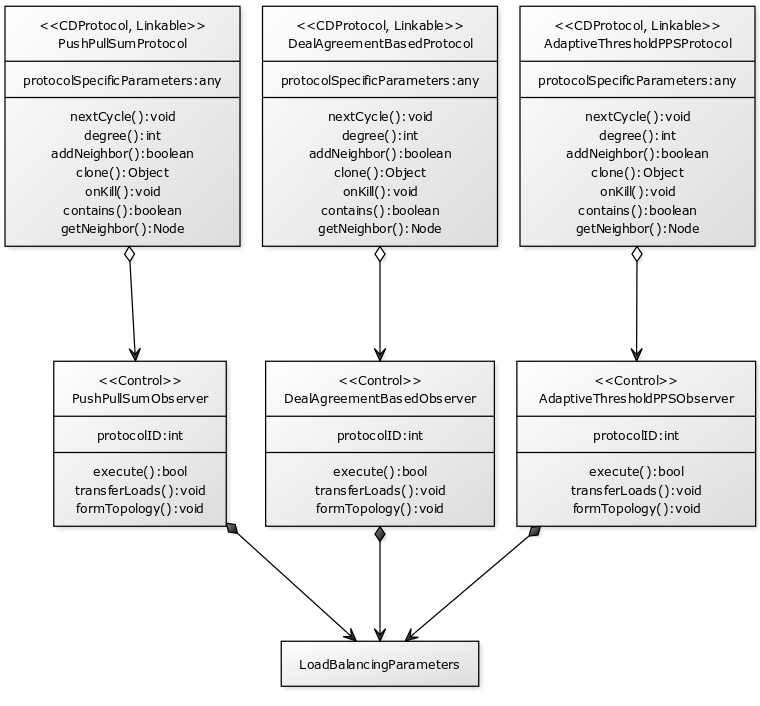
\includegraphics{figures/Diagrams/projectUML.png}}
%     \caption{UML: Project structure}
%     \label{fig:uml}
% \end{figure}

\section{Implementation Details}\label{sec:implementationdetails}
Figure \ref{fig:ProcessModel} depicts a process model, modelling the methodic chosen to get from the creation of experiments to the plots and data analysis part. First I wrote a Python script that generates configuration files where each node has uniformly distributed random load/sum values. 50 distinct experiments were created to improve statistical significance. These configuration files are read with a Java script and each node is assigned a initial load value. Then the simulations are conducted. Each simulation outputs a file containing the simulation results, mainly the mean squared error per round, the loads per round and the configuration of the network (e.g. which topology chosen, network size...). The simulation results are averaged per round and then analyzed. Out of the simulation results plots are generated, showing the mean squared error reduction per round in log-log or log-linear graphs. Also the technique of model fitting is applied.

% \begin{figure}
%     \centering
%     \scalebox{0.38}{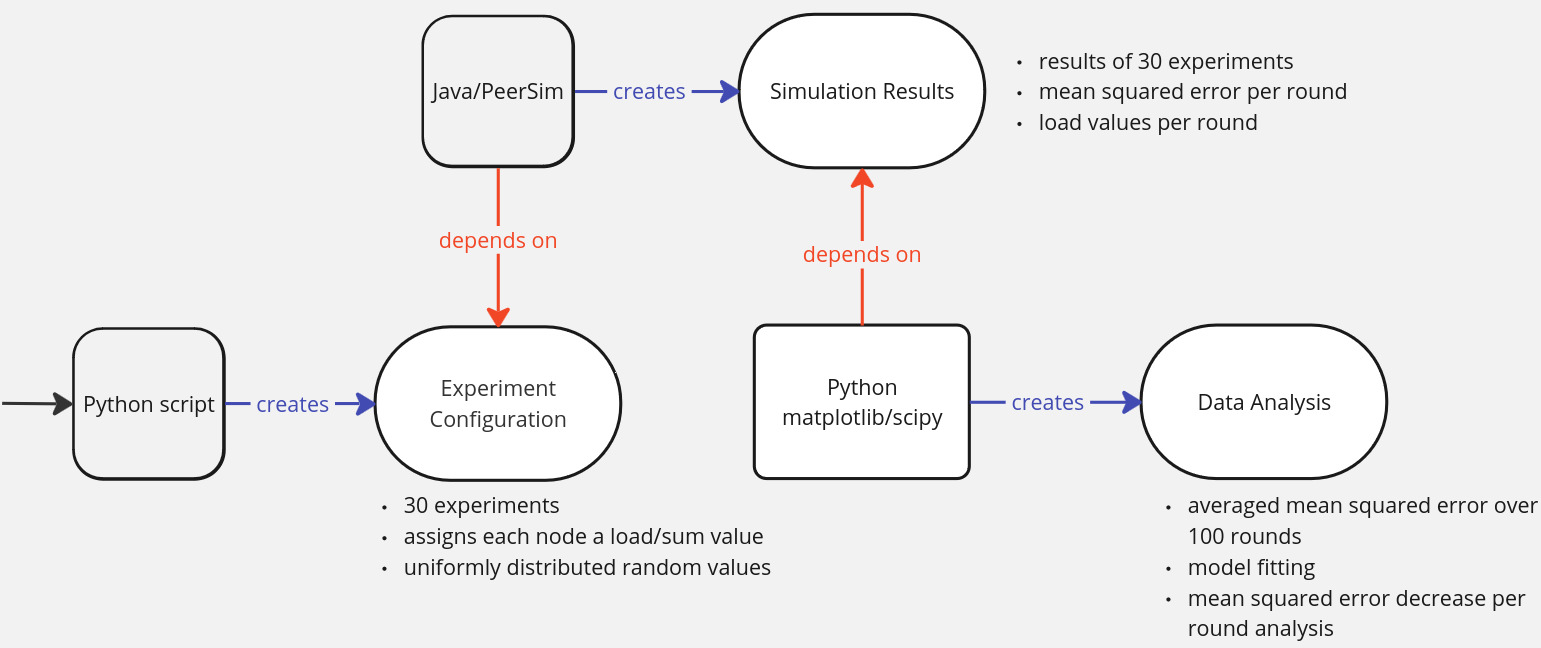
\includegraphics{figures/Diagrams/process_model.png}}
%     \caption{Process Model: Methodic}
%     \label{fig:ProcessModel}
% \end{figure}